\documentclass[fr]{../../../../../../eplexam}
\usepackage{../../../../../../eplunits}
\usepackage{enumitem}
\usepackage{subcaption}
\sisetup{per-mode=symbol}

\hypertitle{Mécanique}{1}{FSAB}{1201}{2017}{Janvier}
{Marius Dechamps \and Thomas Gasòs \and Guillaume Prieur}% \footnote{Avec la relecture et les corrections de Jean-Martin Vlaeminck} }
{Roland Keunings et Jean-Didier Legat}

% Question 1
\section{}
Vous désirez faire monter une roue de vélo de masse $m$ et de rayon $R$ en haut d'une marche de hauteur $h$. Pour ce faire, vous appliquez une force $\vec{F}$ (figure \ref{fig:q1}). Quelle est la plus petite magnitude de la force $\vec{F}$ nécessaire afin de réussir à monter la roue en haut de la marche si la force est appliquée 
(a) au centre de la roue et
(b) au sommet de la roue ?
(c) Dans quel cas la force requise est-elle la plus faible ?
\begin{figure}[ht]
	\centering
	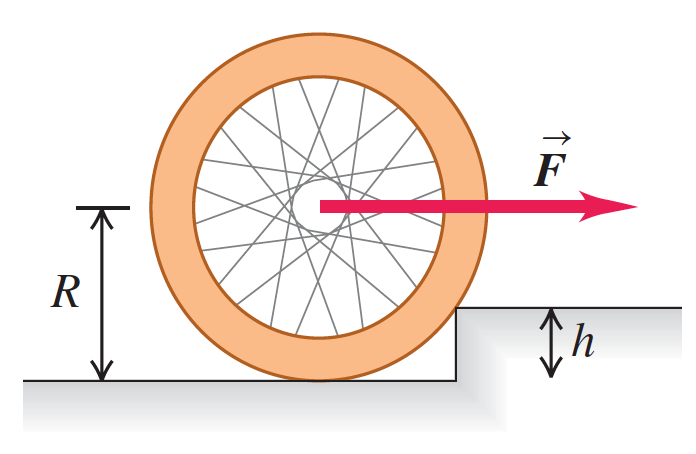
\includegraphics[scale = 0.5]{Question1}
	\caption{Roue de la question 1}
	\label{fig:q1}
\end{figure}

\begin{solution}
Dans la suite, nous notons $A$ le coin supérieur gauche de la marche d'escalier, pris comme point de référence (pivot) par rapport auquel les moments de forces seront déterminés.
\begin{enumerate}[label=(\alph*)]
	\item Lorsque la force $\vec{F}$ est appliquée, la roue est à l'équilibre, et il n'y a plus aucune force de contact entre la roue et la marche inférieure. Nous avons donc nécessairement $\sum \vec{\tau} = 0$ autour de $A$. Dès lors, la force $\vec{F}$ agit avec un bras de levier $(R-h)$ (distance entre le point d'application de la force et le point de référence, mesurée perpendiculairement à la force) % pas tout à fait sûr de la définition de bras de levier dans ce cas.
	et le poids $\vec{P}$ agit avec un brase de levier $\sqrt{R^2-(R-h)^2} = \sqrt{2Rh - h^2}$. Le moment de force total autour de $A$ est donc $\sum \tau = mg\sqrt{2Rh-h^2} - F(R-h)$ (dans l'axe de la roue), et en imposant que ce moment soit nul afin de garantir l'équilibre, nous avons
	\[F = mg\frac{\sqrt{2Rh - h^2}}{R-h}\]
	\item Le moment de force dû à la gravité est le même tandis que la force $\vec{F}$ a cette fois un bras de levier de $(2R-h)$.
	Par l'équilibre nous obtenons,
	\[F = mg\frac{\sqrt{2Rh - h^2}}{2R-h}\]
	\item La force minimale requise est celle appliquée au sommet de la roue quand la distance entre le pivot et la force $\vec{F}$ est la plus grande.
\end{enumerate}
\end{solution}

% Question 2
\section{}
Considérons un mobile de masse $m$ dans un mouvement circulaire uniforme de rayon $R$. (a) Quelle est sa vitesse maximale lorsqu'il se déplace sur un tournant plat avec un frottement pneu-route (figure \ref{fig:q2_1}) ? (b) Quelle est sa vitesse maximale lorsqu'il se déplace sur un tournant penché d'un angle $\beta$ en considérant qu'il n'y ait aucun frottement (figure \ref{fig:q2_2}) ? Justifier.
\begin{figure}[ht]
	\centering
	\begin{subfigure}[b]{.40\linewidth}
		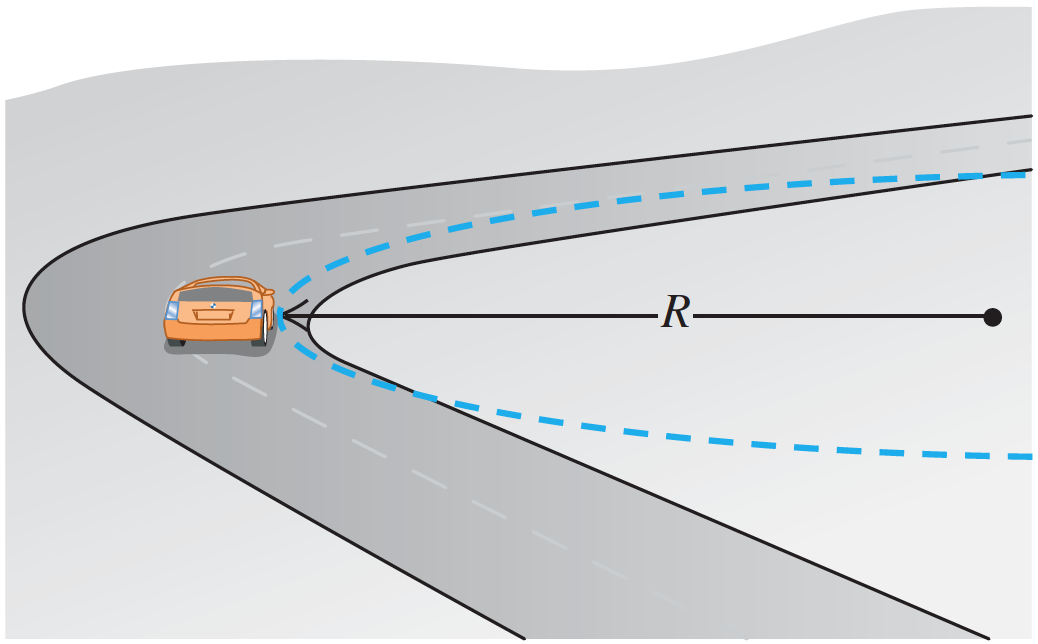
\includegraphics[scale = 0.32]{Question2a}
		\caption{Mobile sur plan horizontal, frottements.}
		\label{fig:q2_1}
	\end{subfigure}
	\begin{subfigure}[b]{.40\linewidth}
		\centering
		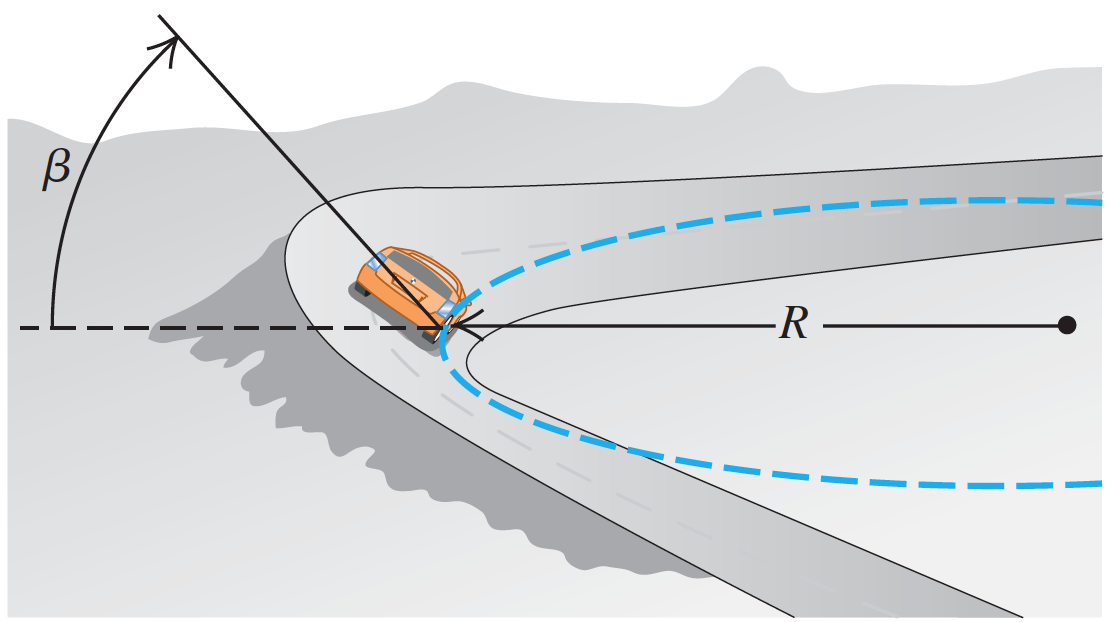
\includegraphics[scale = 0.32]{Question2b}
		\caption{Mobile sur plan incliné, sans frottement.}
		\label{fig:q2_2}
	\end{subfigure}
	\caption{Mobile de la question 2}
	\label{fig:q2_a}
\end{figure}

\begin{solution}
Dans la suite, nous prenons la convention que les vecteurs horizontaux (dénotés par l'indice $x$) sont positifs lorsqu'ils sont dirigés vers le centre de la courbure, et que les vecteurs verticaux (indice $z$) sont positifs lorsqu'ils pointent vers le haut. On définit aussi les vecteurs dits unitaires $\hat{x}$ et $\hat{z}$, dirigés dans les directions précisées.

\begin{enumerate}[label=(\alph*)]
	\item Le mobile subit trois forces :
	\begin{itemize}
		\item son poids, $\vec{P}=-mg \hat{z}$, dirigé vers le centre de la terre ;\footnote{On considère $g>0$ même si rigoureusement, $\vec{g}$ pointe déjà vers le bas et $g$ devrait être négatif. Cela reste une question de convention de signes.} % Bon, la note de bas de page se retrouve à la fin de la minipage, et pas en bas de la vraie page. Faudra corriger ça.
		\item la force normale $\vec{N} = N \hat{z}$ exercée sur le mobile par la route ;
		\item le frottement $\vec{f} = \mu_s N \hat{x}$ exercé par la route, et dirigé vers le centre de la courbe. Le frottement est statique car la voiture ne glisse pas latéralement dans la courbe (elle ne dérape pas) ; dès lors, même si les roues sont en mouvement, le coefficient à prendre en compte est celui du frottement statique.\footnote{En fait, tant que la roue est en roulement sans glissement, les coefficients à prendre en compte sont les coefficients statiques car le point de contact de la roue est localement immobile par rapport à la route.}
	\end{itemize}
	L'accélération dans l'axe vertical étant nul (la voiture ne décolle pas à priori), et l'accélération centripète étant $\vec{a} = \frac{v^2}{R} \hat{x}$, nous pouvons écrire la deuxième loi de Newton dans les directions $\hat{x}$ et $\hat{z}$ :
	\[\begin{cases}
	P+N = -mg + N &= 0 \\
	f = \mu_s N &= m\frac{v^2}{R} \\
	\end{cases}\]
	De la première équation, on tire $N=mg$, que l'on peut dès lors injecter dans la seconde équation :
	\begin{align*}
	f = \mu_s mg &= m\frac{v^2}{R} \\
	v^2 &= \mu_s R g \\
	\end{align*}
	et donc
	\[ v = \sqrt{\mu_s R g} \]
	\item Le mobile subit deux forces :
	\begin{itemize}
		\item son poids, $\vec{P}=-mg \hat{z}$, pointant vers le bas ;
		\item la force normale exercée par la route, $\vec{N} = N_x \hat{x} + N_z \hat{z} = N \sin(\beta) \hat{x} + N \cos(\beta) \hat{z}$ ;
	\end{itemize}
	Dans les deux directions $\hat{x}$ et $\hat{z}$, la deuxième loi de Newton doit être satisfaite. Comme $a_z = 0$ et $a_x = a_\mathrm{rad}$, on a
	\[\begin{cases}
	P+N_z = -mg + N \cos(\beta) &= 0 \\
	N_x = N \sin(\beta) &= m a_\mathrm{rad} = m \frac{v^2}{R} \\
	\end{cases}\]
	De ces équations, on trouve (en remplaçant $m$)
	\begin{align*}
	a_\mathrm{rad} &= \frac{N\sin(\beta)}{m} \\
	&= \frac{N\sin(\beta)}{N\cos(\beta)} g \\
	\frac{v^2}{R} &= g \tan(\beta) \\
	v^2 &= gR \tan(\beta) \\
	\end{align*}
	et finalement,
	\[ v=\sqrt{gR \tan \beta} \]
\end{enumerate}
\end{solution}

% Question 3
\section{}
Considérons une table à coussin d'air. Nous lançons un palet A d'une masse de \SI{0.25}{\kilogram} à une vitesse initiale $v_i$ dans la direction d'un autre palet B d'une masse de \SI{0.35}{\kilogram} au repos. Après la collision, le palet A va à \SI{0.12}{\meter\per\second} vers la gauche tandis que le palet B va à \SI{0.65}{\meter\per\second} vers la droite. Est-ce une collision élastique ? Justifier.

\begin{solution}
Tout au long de l'exercice, une vitesse sera considérée positive si l'objet se meut vers la droite.

Cette collision est inélastique car il n'y a pas de conservation d'énergie mécanique totale. En effet calculons la vitesse initiale du palet A, via la conservation de la quantité de mouvement :
\[m_{A} \cdot v_{i}= m_{A} \cdot v_{A} + m_{B} \cdot v_{B}\]
\begin{align*}
v_{i} &= \frac{0.25 \cdot (-0.12) + 0.35 \cdot 0.65}{0.25} \\
&= \SI{0.79}{\meter\per\second} \\
\end{align*}
Et la vitesse initiale vaut
\[v_{1} = 0.79 \text{ m/s}\]
Afin de déterminer si la collision est inélastique ou non, vérifions la conservation de l'énergie mécanique :
\[E_i = \frac{m_{A}v_{i}^2}{2} \simeq \SI{0.0780}{\joule}\]
tandis que
\[E_f = \frac{m_{A}v_{A}^2}{2} + \frac{m_{B}v_{B}^2}{2} = \SI{0.0757}{\joule}\]
\[0.078=0.0018+0.0739\]
Comme $E_f<E_i$, il y a eu une perte d'énergie mécanique (convertie par exemple en chaleur, son, déformation...), et la collision n'est pas élastique.
\end{solution}

% Question 4
\section{}
Un satellite suit une trajectoire elliptique autour d'un astre.
\begin{enumerate}[label=(\alph*)]
	\item A quel moment sa vitesse croît-elle ?
	\item A quel moment décroît-elle ?
	\item Quand atteint-il sa vitesse maximale ?
	\item Quand atteint-il sa vitesse minimale ?
\end{enumerate}
(Quand nous parlons de vitesse, nous faisons référence à la norme de la vitesse vue par l'astre dans un repère considéré galiléen.)
\begin{figure}[ht]
	%TODO faire un schéma tikz
	\centering
	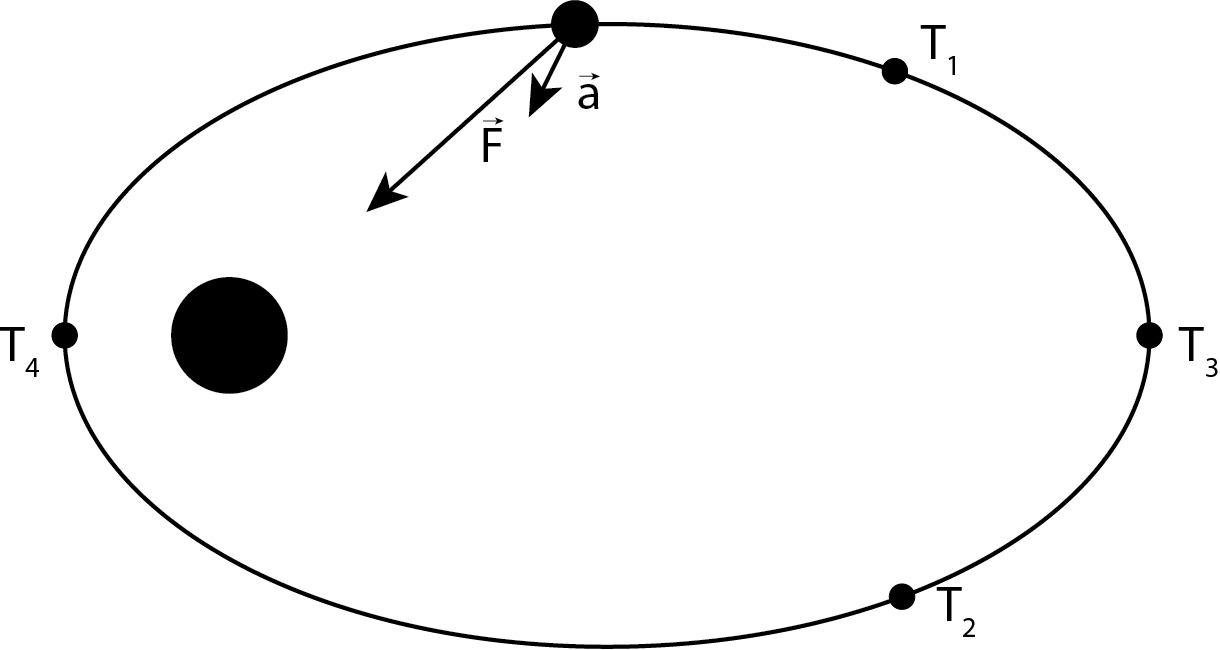
\includegraphics[scale=0.8]{Question4.png}
	\caption{Satellite en rotation autour d'un astre}
	\label{fig_q4}
\end{figure}

\begin{solution}
Tout au long de l'exercice, nous négligerons les forces extérieures dues à d'autres planètes. Dès lors, la seule force agissant sur le satellite est la force gravitationnelle de l'astre. Étant donné que nous sommes dans un repère galiléen, nous pouvons appliquer les lois de Newton sur ce phénomène.

\begin{enumerate}[label=(\alph*)]
	\item Nous voyons sur la figure \ref{fig_q4}, que l'unique force au temps T1, se dirige vers l'astre. Par Newton, nous pouvons affirmer que son accélération aussi ($\sum{\vec{F}}=m\vec{a}$). Nous voyons que l'accélération a une composante tangentielle ayant la même direction que la vitesse. Le satellite accélère.
	\item Au temps T2, la composante tangentielle de l'accélération est de sens opposé au vecteur vitesse. Le satellite ralenti.
	\item Au temps T3, la composante tangentielle de l'accélération est nulle. Le satellite finit de ralentir pour commencer à accélérer. Il a atteint sa vitesse minimale.
	\item Au temps T4, le satellite finit d'accélérer et commence à ralentir. Il a atteint sa vitesse maximale.
\end{enumerate}

\end{solution}

\section*{Partie électricité}
La partie électricité de l'examen se trouve dans le dossier dédié (Synthèses-EPL > q1 > elec-FSAB1201 > exam > 2017\_Janvier).

\end{document}
